\documentclass[landscape]{article}
\usepackage[landscape,margin=0.7in]{geometry}
\usepackage{pgfplots}
\usepackage{tikz}
\pgfplotsset{compat=1.18}

\begin{document}
\pagestyle{empty}

\begin{figure}
    \centering
    \begin{tikzpicture}
        \begin{axis}[
            title={\Large Hybrid Strategy - COMPLETE (All passengers seated)},
            xlabel={Seat Column},
            ylabel={Row Number},
            xticklabels={A,B,C,D,E,F},
            ytick={1,2,3,4,5,6,7,8,9,10,11,12,13,14,15,16,17,18,19},
            xtick={0,1,2,3,4,5},
            xmin=-0.5,
            xmax=5.5,
            ymin=0.5,
            ymax=19.5,
            y dir=reverse,
            enlargelimits=false,
            axis on top,
            width=0.9\textwidth,
            height=0.4\textheight,
            colorbar,
            colormap={boarding}{
                color(0)=(white);
                color(0.5)=(yellow);
                color(1)=(purple)
            },
            colorbar style={
                title={Status},
                ytick={0,0.5,1},
                yticklabels={Empty,Boarding,Seated},
            },
            point meta min=0,
            point meta max=1
        ]
            
        % All seats occupied (1)
        \addplot[matrix plot, mesh/cols=6, point meta=explicit] table [meta=C] {
            x y C
            0 1 1
            1 1 1
            2 1 1
            3 1 1
            4 1 1
            5 1 1
            0 2 1
            1 2 1
            2 2 1
            3 2 1
            4 2 1
            5 2 1
            0 3 1
            1 3 1
            2 3 1
            3 3 1
            4 3 1
            5 3 1
            0 4 1
            1 4 1
            2 4 1
            3 4 1
            4 4 1
            5 4 1
            0 5 1
            1 5 1
            2 5 1
            3 5 1
            4 5 1
            5 5 1
            0 6 1
            1 6 1
            2 6 1
            3 6 1
            4 6 1
            5 6 1
            0 7 1
            1 7 1
            2 7 1
            3 7 1
            4 7 1
            5 7 1
            0 8 1
            1 8 1
            2 8 1
            3 8 1
            4 8 1
            5 8 1
            0 9 1
            1 9 1
            2 9 1
            3 9 1
            4 9 1
            5 9 1
            0 10 1
            1 10 1
            2 10 1
            3 10 1
            4 10 1
            5 10 1
            0 11 1
            1 11 1
            2 11 1
            3 11 1
            4 11 1
            5 11 1
            0 12 1
            1 12 1
            2 12 1
            3 12 1
            4 12 1
            5 12 1
            0 13 1
            1 13 1
            2 13 1
            3 13 1
            4 13 1
            5 13 1
            0 14 1
            1 14 1
            2 14 1
            3 14 1
            4 14 1
            5 14 1
            0 15 1
            1 15 1
            2 15 1
            3 15 1
            4 15 1
            5 15 1
            0 16 1
            1 16 1
            2 16 1
            3 16 1
            4 16 1
            5 16 1
            0 17 1
            1 17 1
            2 17 1
            3 17 1
            4 17 1
            5 17 1
            0 18 1
            1 18 1
            2 18 1
            3 18 1
            4 18 1
            5 18 1
            0 19 1
            1 19 1
            2 19 1
            3 19 1
            4 19 1
            5 19 1
        };
        
        % Draw aisle line
        \draw[black, thick, dashed] (axis cs:2.5,0.5) -- (axis cs:2.5,19.5);
        
        % Draw zone boundaries
        \draw[black, thick] (axis cs:-0.5,6.5) -- (axis cs:5.5,6.5);  % Front-Middle boundary
        \draw[black, thick] (axis cs:-0.5,12.5) -- (axis cs:5.5,12.5);  % Middle-Back boundary
        
        % Add zone labels
        \node[right] at (axis cs:5.5,3.5) {Front Zone (Rows 1-6)};
        \node[right] at (axis cs:5.5,9.5) {Middle Zone (Rows 7-12)};
        \node[right] at (axis cs:5.5,16) {Back Zone (Rows 13-19)};
        
        % Time indicator
        \node[font=\Large] at (axis cs:2.5,20.5) {t = 20 minutes - BOARDING COMPLETE};
        
        % Legend
        \node[draw, align=left, anchor=south west] at (axis cs:-0.5,-2) {
            \textbf{Boarding Sequence:}\\
            \textcolor{purple}{Step 1: Back Window Seats (Rows 13-19, Seats A \& F) - COMPLETE}\\
            \textcolor{purple}{Step 2: Middle Window Seats (Rows 7-12, Seats A \& F) - COMPLETE}\\
            \textcolor{purple}{Step 3: Front Window Seats (Rows 1-6, Seats A \& F) - COMPLETE}\\
            \textcolor{purple}{Step 4: Back Middle Seats (Rows 13-19, Seats B \& E) - COMPLETE}\\
            \textcolor{purple}{Step 5: Middle Middle Seats (Rows 7-12, Seats B \& E) - COMPLETE}\\
            \textcolor{purple}{Step 6: Front Middle Seats (Rows 1-6, Seats B \& E) - COMPLETE}\\
            \textcolor{purple}{Step 7: Back Aisle Seats (Rows 13-19, Seats C \& D) - COMPLETE}\\
            \textcolor{purple}{Step 8: Middle Aisle Seats (Rows 7-12, Seats C \& D) - COMPLETE}\\
            \textcolor{purple}{Step 9: Front Aisle Seats (Rows 1-6, Seats C \& D) - COMPLETE}
        };
        \end{axis}
    \end{tikzpicture}
\end{figure}

\begin{figure}
    \centering
    \begin{tikzpicture}
        \begin{axis}[
            title={\Large Hybrid Strategy - Boarding Time Improvement},
            xlabel={Boarding Strategy},
            ylabel={Average Boarding Time (minutes)},
            symbolic x coords={Random, Back-to-Front, Outside-In, Hybrid},
            xtick=data,
            ybar,
            ymin=0,
            ymax=25,
            bar width=25pt,
            nodes near coords,
            nodes near coords align={vertical},
            width=0.8\textwidth,
            height=0.4\textheight,
            enlarge x limits=0.25,
            legend pos=north east,
            colormap/hot
        ]
            
            \addplot[fill=red!80!black] coordinates {
                (Random, 18.7)
                (Back-to-Front, 11.2)
                (Outside-In, 7.5)
                (Hybrid, 10.0)
            };
            
            % Add improvement percentages
            \node[above] at (axis cs:Hybrid,10.0) {46.5\% vs Random};
            \node[above, yshift=1.5em] at (axis cs:Hybrid,10.0) {10.7\% vs B-to-F};
            \node[above, yshift=3em] at (axis cs:Hybrid,10.0) {-33.3\% vs Outside-In};
        \end{axis}
    \end{tikzpicture}
    \caption{Performance comparison showing the Hybrid strategy offers significant improvement over Random and Back-to-Front, while being more practical to implement than Outside-In}
\end{figure}

\end{document}